\documentclass{lecturenotes}
\renewcommand{\vecka}{1}


\title[Föreläsningsanteckningar EDA016, 2015]{EDA016 Programmeringsteknik för D}
\subtitle{Läsvecka \vecka: Introduktion}
\author{Björn Regnell}
\institute{Datavetenskap, LTH}
\date{Lp1-2, HT 2015}
 
\begin{document}

\frame{\titlepage}
\setnextsection{\vecka}
\section[Vecka \vecka: Introduktion]{Introduktion}
\frame{\tableofcontents}

%%%%%%%%%%%%%%%%%%%%%%%%%%%%%%%%%%%%%%
\Subsection{Om denna kurs}

%%%
\frame{\frametitle{Vad och hur?}
\begin{itemize}
\item \emph{Vad} ska du lära dig?
\begin{itemize}
\item Grundläggande principer för programmering\\ $\implies$Inga förkunskaper i programmering krävs
\item Konstruktion av enkla algoritmer
\item Tänka i abstraktioner
\item Imperativ och objektorienterad programmering
\item Programspråket Java
\item Utvecklingsmiljön Eclipse: implementera, testa, felsöka
\end{itemize}
\item \emph{Hur} ska du lära dig?
\begin{itemize}
\item Genom praktiskt eget arbete: \Emph{Lära genom att göra!}
\item Genom studier av kursens teori: \Emph{Skapa förståelse!}
\item Genom samarbete med dina kurskamrater: \Emph{Gå djupare!}
\end{itemize}
\end{itemize}}

%%%
\frame{\frametitle{Kurslitteratur}
\begin{columns}
\begin{column}{0.6\textwidth}
\begin{itemize}
\item ''Objektorienterad programmering och Java" av Per Holm
\item Kurskompendium med övningar och laborationer
\item Bokpaket säljs på KFS \\John Ericssons väg 4 \url{http://www.kfsab.se/}
\end{itemize}
\end{column}
\begin{column}{0.5\textwidth}
\centering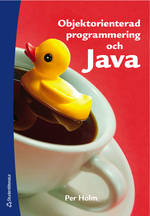
\includegraphics[width=0.5\textwidth]{img/ankbok.jpg}
\end{column}
\end{columns}
}

%%%
\frame{\frametitle{Personal}
%\footnotesize
\Size{9pt}
\begin{description}
\item [\bfseries Kursansvarig:] ~\\Björn Regnell, bjorn.regnell@cs.lth.se
\item [\bfseries Kurssekreterare:]  ~\\Lena Ohlsson \\Exp.tid 09.30 -- 11.30 samt 12.45 -- 13.30
\item [\bfseries Handledare:] ~\\
Maj	Stenmark,	Tekn. Lic., Doktorand\\
Gustav	Cedersjö,	Doktorand\\
Anton	Klarén,	D09\\
Maria	Priisalu	, D11\\
Anders	Buhl,	D13\\
Erik	Bjäreholt,	D13\\
Fatima	Abou Alpha,	D13\\
Cecilia	Lindskog,	D14\\
Emma	Asklund,	D14\\
\end{description}
}

%%%
\frame{\frametitle{Kursmoment --- varför?}\footnotesize
\begin{itemize}
\item \textbf{Föreläsningar}: skapa översikt, ge struktur, förklara teori, svara på frågor, motivera varför
\item \textbf{Övningar}: bearbeta teorin med avgränsade problem som mestadels löses med papper  \& penna, förberedelse inför laborationerna
\item \textbf{Laborationer}: lösa programmeringsproblem praktiskt, obligatoriska uppgifter; lösningar redovisas för handledare
\item \textbf{Resurstider}: få hjälp med övningar och laborationsförberedelser av handledare
\item \textbf{Samarbetsgrupper}: grupplärande genom samarbete och dialog 
\item \textbf{Kontrollskrivning}: obligatorisk, diagnostisk, kamraträttad; kan ge samarbetsbonuspoäng till tentan
\item \textbf{Inlämningsupgift}: du visar att du kan skapa ett större program självständigt; redovisas för handledare
\item \textbf{Tenta}: Skriftlig tentamen utan hjälpmedel, förutom  \href{http://fileadmin.cs.lth.se/cs/Education/EDA016/general/quickref-booklet.pdf}{snabbreferens}.
\end{itemize}
}

%%%
\frame{\frametitle{Nytt för i år }
Årets kurs är i flera avseende väsentligt annorlunda and förra årets upplaga, så lita inte på allt som era äldre kursare säger :) 
\begin{itemize}
\item Övningar blir resurstider i datorsal
\item Inlämningsuppgift utan skriftlig rapport
\item Samarbetskultur och grupplärande
\item Nya övningar 
\item Nya laborationer
\item Nya föreläsningar
\end{itemize}
\vskip1em
{\fontsize{8pt}{9pt}\selectfont  Ändringarna är framtagna i samråd med studierådet. Mer om bakgrunden här: \\ 
\url{http://fileadmin.cs.lth.se/cs/Education/EDA016/2015/update.pdf}}
}

%%%
\frame{\frametitle{Detta är bara början... }
Exempel på efterföljande kurser som bygger vidare på denna:
\begin{itemize}
\item Årskurs 1
\begin{itemize}
\item Programmeringsteknik -- fördjupningskurs
\item Utvärdering av programvarusystem
\item Diskreta strukturer
\end{itemize}
\item Årskurs 2
\begin{itemize}
\item Objektorienterad modellering och design
\item Programvaruutveckling i grupp
\item Algoritmer, datastrukturer och komplexitet
\item Funktionsprogrammering
\end{itemize}
\end{itemize}
}

\begin{Slide}{Utveckling av mjukvara i praktiken}
\begin{itemize}
\item \Emph{Inte bara kodning:} kravbeslut, releaseplanering, design, test, versionshantering, kontinuerlig integration, driftsättning, återkoppling från dagens användare, ekonomi \& investering, gissa om morgondagens användare, ... 
\item \Emph{Teamwork:} Inte ensamma hjältar utan autonoma team i decentraliserade organisationer med innovationsuppdrag
\item \Emph{Snabbhet:} Att koda innebär att hela tiden uppfinna nya ''byggstenar'' som ökar organisationens förmåga att snabbt skapa värde med hjälp av mjukvara. Öppen källkod. Skapa kraftfulla API. 
\item \Emph{Livslångt lärande:} Lär nytt och dela med dig hela tiden. Exempel på pedagogisk utmaning: hjälp andra förstå och använda ditt API $\implies$ \textit{Samarbetskultur}
\end{itemize}
\end{Slide}

%%%
\begin{Slide}{Att skapa koden som styr världen}
\begin{multicols}{2}
I stort sett alla delar av samhället styrs av mjukvara:
{\scriptsize
\begin{itemize}
\item kommunikation
\item transport
\item byggsektorn
\item statsförvaltning
\item finanssektorn
\item media
\item sjukvård
\item övervakning
\item integritet
\item upphovsrätt
\item miljö \& energi
\item sociala relationer
\item utbildning 
\end{itemize}}
\columnbreak %---------
Hur blir ditt framtida yrkesliv som systemutvecklare?
{\Size{8pt}
\begin{itemize}
\item  Redan nu är det en skriande brist på utvecklare och bristen blir bara värre och värre... \\
  \href{http://computersweden.idg.se/2.2683/1.634770/rekrytera-utvecklare}{CS 2015-08-17}
\item Global kompetensmarknad \\ 
  \href{http://computersweden.idg.se/2.2683/1.630901/det-finns-programmerare-och-sa-finns-det-programmerare}{CS 2015-06-14}\\
   \href{http://computersweden.idg.se/2.2683/1.634700/7-satt-att-bli-en-battre-programmerare}{CS 2015-08-15}
\item Fokus på innovation, tid-till-marknad
\item Autonoma utvecklingsteam i decentraliserade organisationer
\item Öppen källkod
\end{itemize}}
\end{multicols}
\end{Slide}
%%%

\frame{\frametitle {Registrering}
\begin{itemize}
\item Fyll i listan som jag skickar runt.
\item Kryssa i kolumnen \Emph{Ska gå} om du ska gå kursen\footnote{Redan gått motsvarande högskolekurs? Ansök då om tillgodoräknande}
\item Kryssa i kolumnen \Emph{Programmerat} om du har programmerat innan (även om bara lite grand) 
\item Kryssa i kolumnen \Emph{Kursombud} om du kan tänka dig att vara kursombud under kursens gång
\begin{itemize}
\item Alla LTH-kurser ska utvärderas under kursens gång och efter kursens slut.
\item Till det behövs kursombud -- ungefär 2 D-are och 2 W-are.
\item Ni kommer att bli kontaktade av studierådet.
\end{itemize}
\end{itemize}
}

%%%
\begin{Slide}{Förkunskaper}
\begin{itemize}
\item Förkunskaper $\neq$ Förmåga
\item Varken kompetens eller personliga egenskaper är statiska 
\item ''Programmeringskompetens'' är inte \textit{en} enda enkel förmåga utan en komplex sammansättning av flera olika förmågor som utvecklas genom hela livet
\item Ett innovativt utvecklar\Emph{team} behöver många olika kompetenser för att vara framgångsrikt
\end{itemize}
\end{Slide}

\SlideImg{Stor spridning i programmeringsförkunskaper \\ bland D-are (enl. enkätsvar 2010-2014)}{img/pre-pie}

%%%
\frame{\frametitle{Förkunskapsenkät}
Fyll i denna enkät på rasten (eller senast ikväll kl 20:00) \\
\url{http://cs.lth.se/eda016/survey} 
\vskip1em
Ligger till grund för randomiserad gruppindelning,\\ så att det blir en spridning av förkunskaper inom gruppen.
}

%%%
\begin{Slide}{Samarbetgrupper}\footnotesize
\begin{itemize}
\item Ni delas in i \Emph{samarbetsgrupper} om ca 5 personer baserat på förkunskapsenkäten, så att olika förkunskapsnivåer sammanförs
\item 2 av de 11 laborationerna är mer omfattande \Emph{grupplabbar} och kommer att göras i samarbetsgrupperna (Lab 9 och 11 i Lp2) \\ \vspace{1em}
\item Kontrollskrivningen i halvtid kan ge \Emph{samarbetsbonus} (max 3p) som adderas till ordinarie tentans poäng (max 45p) med medelvärdet av gruppmedlemmarnas individuella kontrollskrivningspoäng 
\scriptsize \parbox{7cm}{Bonus $b$ för varje person i en grupp med $n$ medlemmar med $p_i$ poäng vardera på kontrollskrivningen:} 
 \hspace{5mm} $\displaystyle b = \sum\limits_{i=1}^n \frac{p_i}{n}$
\end{itemize}
\end{Slide}

%%%
\begin{Slide}{Varför samarbetsgrupper?}

Huvudsyfte: \Emph{Djupinlärning!}

\begin{itemize}
\item Pedagogisk forskning stödjer tesen om att lärandet fördjupas om det sker i utbyte med andra
\item Ett studiesammanhang med höga ambitioner och respektfull gemenskap gör att vi \Emph{når mycket längre}
\item Varför ska du som redan kan mycket aktivt dela med dig av dina kunskaper?
\begin{itemize}
\item Förstå bättre själv genom att förklara för andra
\item Träna din pedagogiska förmåga
\item Förbered dig för inför ditt kommande yrkesliv som mjukvaruutvecklare 
\end{itemize}
\end{itemize}
\end{Slide}

%%%
\begin{Slide}{Samarbetskontrakt}
Gör ett skriftligt samarbetskontrakt med dessa och ev. andra punkter som ni också tycker bör ingå:
\begin{enumerate}
\item Kom i tid till gruppmöten
\item Var väl förberedd genom självstudier inför gruppmöten
\item Hjälp varandra att förstå, men ta inte över och lös allt
\item Ha ett respektfullt bemötande även om ni har olika åsikter
\item Inkludera alla i gemenskapen
\end{enumerate}

Diskutera hur ni ska uppfylla dessa innan alla skriver på. \\ Ta med samarbetskontraktet och visa för handledare på labb 1.

\vskip1em

\textcolor{red}{Om arbetet i samarbetsgruppen inte fungerar ska ni mejla kursansvarig och boka mötestid!}
\end{Slide}

\begin{Slide}{Bestraffa inte frågor!}
\begin{itemize}
\item Det finns bättre och sämre frågor vad gäller hur mycket man kan lära sig av svaret, men \Emph{all undran är en chans} att i dialog utbyta erfarenheter och lärande
\item Den som frågar \Emph{vill veta} och berättar genom frågan något om nuvarande kunskapsläge
\item Den som svarar får chansen att \Emph{reflektera} över vad som kan vara svårt och olika vägar till djupare förståelse
\item I en hälsosam lärandemiljö är det \Emph{helt tryggt} att visa att man ännu inte förstår, att man gjort ''fel'', att man har mer att lära, etc. 
\item Det är viktigt att våga försöka även om det blir ''fel'':\\ \Emph{det är ju då man lär sig!}
\end{itemize}
\end{Slide}

%%%
\begin{Slide}{Plagiatregler}
Läs dessa regler noga och diskutera i samarbetsgrupperna:
\begin{itemize}
\footnotesize
\item \url{http://cs.lth.se/utbildning/samarbete-eller-fusk/}
\item \url{http://cs.lth.se/utbildning/foereskrifter-angaaende-obligatoriska-moment/}
\end{itemize}
Ni ska lära er genom \Emph{eget arbete} och genom  \Emph{bra samarbete}. Samarbete gör att man lär sig bättre, men man lär sig inte av att bara kopiera andras lösningar. Plagiering är förbjuden och kan medföra disciplinärende och avstängning.
\end{Slide}

%%%
\frame{\frametitle{En typisk kursvecka}
\begin{itemize}
\item Gå på föreläsningar måndag--tisdag
\item Jobba själv med boken, övningar, labbförberedelser
\item Träffas i samarbetsgruppen och hjälp varandra att förstå mer och fördjupa lärandet
\item Gå till resurstider och få hjälp och tips av handledare, onsdag--torsdag
\item Genomför obligatorisk laboration på fredagen
\end{itemize}
Se detaljerna och undantagen i \href{http://cs.lth.se/eda016/schema}{schemat i TimeEdit}
}

%%%
\begin{Slide}{Resurstider}
\begin{itemize}
\item På resurstiderna får du hjälp med övningar och laborationsförberedelser
\item Kom till minst en resurstid per vecka (se \href{http://cs.lth.se/eda016/schema/}{schema})
\item Handledare gör ibland genomgångar för alla under resurstiderna
\end{itemize}
\end{Slide}

%%%
\begin{Slide}{Laborationer}\footnotesize
\begin{itemize}
\item \textcolor{red}{Programmering lär man sig bäst genom att programmera ... }
\item Labbarna är \Emph{individuella} (utom 2) och \Emph{obligatoriska}
\item Gör förberedelserna noga \textit{innan} själva labben -- detta är ofta helt nödvändigt för att du ska hinna klart
\item Är du sjuk? Anmäl det \textit{före} labben till \url{bjorn.regnell@cs.lth.se}, få hjälp på resurstillfällena och redovisa på resurstid eller uppsamlingstid (helst inte på ordinarie tillfälle, men det är OK om handledaren har tid)
\item Hinner du inte med hela? Se till att handledaren noterar din närvaro, och fortsätt på resurstid och uppsamlingstid.
\item Läs noga anvisningarna i kompendiet
\end{itemize}
\end{Slide}



%%%
\frame{\frametitle{Att göra i Vecka 1: Rivstarta}
\begin{enumerate}
\item Läs följande kapitel i kursboken: \\ 1, 3.1-3.3, 5.1-5.3, 6.1-6.2, 7.1-7.3, 7.5-7.6, 7.8-7.9
\item Gör övning 1: Hello World, Hello Args, javac, editera--kompilera--exekvera--felsök, värden, uttryck variabler och tilldelning
\item Gör förberedelserna till laboration 1: skapa textfil, etc.
\item Träffas i samarbetsgrupper och hjälp varandra att förstå
\item Kom till \Emph{resurstiderna} och få hjälp och tips
\item Genomför laboration 1: Quiz --- träna på att editera, läsa, ändra och felsöka i färdig programkod\\ \lstinline{while}, \lstinline{for}, \lstinline{Scanner}
\end{enumerate}
}

%%%%%%%%%%%%%%%%%%%%%%%%%%%%%%%%%%%%%%
%\subsection{Vad är programmering?}

%%%
\Subsection{Vad är programmering?}

%%%
%\frame[plain]{\frametitle{Programming unplugged}
%\centering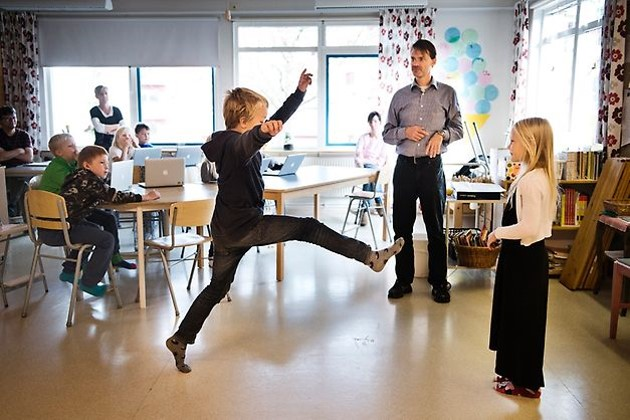
\includegraphics[width=1.0\textwidth]{img/unplugged.jpg}
%}
\SlideImg{Programming unplugged: Två frivilliga?}{img/unplugged}
\SlideImg{Editera och exekvera ett program}{img/kojo}


\begin{SlideSimple}{Världens första programmerare}
\begin{multicols}{2}
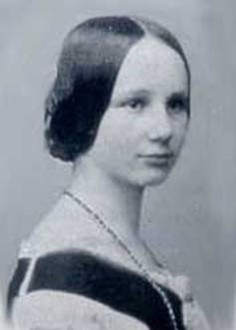
\includegraphics[width=\columnwidth]{img/ada}

\columnbreak %---------

\href{http://kartor.lund.se/wiki/lundanamn/index.php/Ada_Lovelace-parken}{Ada Lovelace} skrev världens första datorprogram på 1800-talet. 
\vskip1em
Programmet skulle köra på en kugghjulsdator som hennes kompis Charles Babbage försökte bygga.
\end{multicols}
\end{SlideSimple}

\SlideImg{Vad är en \href{https://en.wikipedia.org/wiki/ENIAC}{dator}?}{img/eniac}

\begin{SlideSimple}{Vad är en kompilator?}
\begin{multicols}{2}
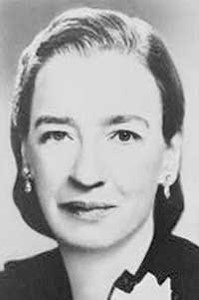
\includegraphics[width=\columnwidth]{img/grace}

\columnbreak %---------

\href{https://en.wikipedia.org/wiki/Grace_Hopper}{Grace Hopper} uppfann första kompilatorn 1952.
\vskip2em
%https://www.sharelatex.com/blog/2013/08/29/tikz-series-pt3.html
\begin{tikzpicture}[node distance=2cm]
\node (input) [startstop] {Källkod};
\node(inptext) [right of=input, text width=2cm, scale=0.8,xshift=1.0cm]{Lättare för människor};
\node (compile) [process, below of=input] {Kompilator};
\node (output) [startstop, below of=compile] {Maskinkod};
\draw [arrow] (input) -- (compile);
\draw [arrow] (compile) -- (output);
\end{tikzpicture}

\end{multicols}
\end{SlideSimple}

\begin{SlideSimple}{Exempel på vanliga programspråk}
\begin{multicols}{2}
\begin{enumerate}
\item  Java
\item C
\item C++
\item C\#
\item Python
\item Objective-C
\item PHP
\item Visual Basic .NET
\item JavaScript
\item Perl
\end{enumerate}

\columnbreak %---------
De 10 ''vanligaste''?
\begin{itemize}
\item \href{http://www.tiobe.com/index.php/content/paperinfo/tpci/index.html}{TIOBE Programming Community Index \\ Augusti 2015}
\item \href{https://github.com/blog/2047-language-trends-on-github}{Språktrender på GitHub 2008-2015}
\end{itemize}
\end{multicols}
\end{SlideSimple}

\frame{\frametitle{Vad är Java?}}

\frame{\frametitle{Utvecklingsverktyg}
Systemutvecklare använder många olika verktyg: \footnotesize
\begin{itemize}
\item kompilator, t.ex. javac
\item editor, t.ex. gedit, Sublime Text 3
\item terminal och kommandoskal, t.ex. bash, powershell
\item integrerad utvecklingsmiljö (eng. Integrated Dev. Environment, IDE), t.ex. \Emph{Eclipse}, IntelliJ
\item versionshanteringssystem, t.ex. git, Mercurial
\item kodlagringsplats, t.ex. GitHub, Bitbucket
\item hypervisor för virtuella maskiner, t.ex. VirtualBox, VMWare
\item bughanteringssystem, t.ex. Bugzilla, Jira
\item byggverktyg, t.ex. Jenkins, Hudson
\item ...
\end{itemize}
}

\frame{\frametitle{Vad är objektorientering?}
\begin{itemize}
\item Det finns många olika \href{https://en.wikipedia.org/wiki/Programming_paradigm}{programmeringsparadigm} (sätt att programmera på), till exempel:
\begin{itemize}\footnotesize
\item \Emph{imperativ programmering:} programmet är uppbyggt av sekvenser av olika satser som påverkar systemets tillstånd
\item \Emph{objektorienterad programmering:} en sorts imperativ programmering där programmet består av objekt som sammanför data och operationer på dessa data
\item \Emph{funktionsprogrammering:} programmet är uppbyggt av samverkande (matematiska) funktioner som undviker föränderlig data och tillståndsändringar  
\item \Emph{deklarativ programmering, logikprogrammering:} programmet är uppbyggt av logiska uttryck som beskriver olika fakta eller villkor och exekveringen utgörs av en bevisprocedur som söker efter värden som uppfyller fakta och villkor
\end{itemize}
\end{itemize}
}

\frame{\frametitle{Grundläggande principer i imperativ programmering}
\footnotesize
\begin{itemize}
\item \Emph{Sekvens}: Ett program innehåller sekvenser av \textit{satser}. Ordningen mellan dessa har helt avgörande betydelse.
\item \Emph{Alternativ}: Systemet reagerar på vad som händer och kan välja olika vägar genom programmet beroende på \textit{variablers} värde\\ Java: \lstinline{if}-sats, \lstinline{switch}-sats
\item \Emph{Repetition}: Göra saker om och om igen\\ Java: \lstinline{while}-loop, \lstinline{for}-loop
\item \Emph{Abstraktion}: Kapsla in (komplexa) programdelar och sätta namn på dessa så att de enkelt går att återanvända utan att att vi behöver ''rota i inanndömet''.\\Java: klasser och metoder  
\end{itemize}
}

%%%%%%%%%%%%%%%%%%%%%%%%%%%%%%%%%%%%%%
\subsection{Vårt första Java-program}
  
%%%
\begin{frame}[fragile]
\frametitle{Hello World!}
\scriptsize Vårt första Java-program i filen \lstinline{HelloWorld.java}
\lstinputlisting[language=Java]{../examples/terminal/hello/HelloWorld.java}

Kompilera och kör:

\begin{lstlisting}[language=bash, backgroundcolor=\color{black!90}, basicstyle=\ttfamily\scriptsize\selectfont\color{white}]
> javac HelloWorld.java
> java HelloWorld
Hej och välkomna!
>
\end{lstlisting}
Ovan ingår i övning 1.
\end{frame}

%%%
\frame{\frametitle{Hello World! -- Vad betyder egentligen allt detta?}
\lstinputlisting[language=Java]{../examples/terminal/hello/HelloWorld.java}
\scriptsize
\begin{itemize}
\item \lstinline{public} Denna programdel är synlig ''utåt'' och kan användas av andra delar.
\item \lstinline{class} Ett slags "kodbyggblock" som samlar olika programdelar. All java-kod måste finnas i en klass. Det finns tusentals färdiga klasser att använda direkt i Java och man kan lätt skapa egna klasser. Klammerpar \{ \} anger början och slut.
\item \lstinline{static} Denna programdel skapas direkt vid programmets start och det finns exakt \emph{en} sådan här per klass.
\item \lstinline{void} Berättar för kompilatorn att inget värde returneras från denna programdel.
\item \lstinline{main} Berättar var exekveringen av programmet börjar.
\item \lstinline{( )} Parentespar berättar för kompilatorn att vi här kan ha parametrar.
\item \lstinline{String[] args} Möjliggör indata till programmet i form av flera textsträngar. Parametern \lstinline{args} måste finnas i \lstinline{main}, men vi använder den inte i detta program. 
\item \lstinline{System.out.println} Den färdiga klassen \lstinline{System} kan bl.a. skriva ut text. Textsträngar avgränsas av citationstecken. Semikolon avgränsar satser.
\end{itemize}
}

%%%%%%%%%%%%%%%%%%%%%%%%%%%%%%%%%%%%%%
\subsection{Grundläggande programkonstruktioner i Java}

%%%
\frame{\frametitle{Några grundläggande delar i ett Javaprogram}
\scriptsize
\begin{itemize}
\item värde (value): data som programmet kan använda \\ 
\lstinline{42}  \hspace{5mm}  \lstinline{"hej"} \hspace{7mm} \lstinline{42.0} \hspace{9mm} \lstinline{true} 
\item uttryck (expression): data kombineras med operatorer och ger nya värden \\ 
\lstinline{41+1}  \hspace{2mm}  \lstinline{"h"+"ej"} \hspace{2mm} \lstinline{43.5-1.5} \hspace{2mm} \lstinline{!false} 
\item deklaration av variabel (variable declaration): skapa plats i minnet för data \\ \lstinline{int x = 42;}
\item tilldelningssats (assignment): ändra värdet på variabler \\ \lstinline{x = 43;}
\item alternativ (choice): välj väg beroende på variablers värde \\ \lstinline{if  switch}
\item repetition (loop): upprepa om och om igen \\ \lstinline{while  for}
\end{itemize}
}

\frame{\frametitle{Värden och uttryck}
%\lstinputlisting[language=Java]{../examples/terminal/expressions/Expressions.java}
}

\begin{Slide}{Alternativ}
\footnotesize
Välj väg genom programmet med \lstinline{if}-sats.
\lstinputlisting[language=Java]{../examples/terminal/alternative/Alternative.java}
En if-sats gör så att exekveringen av programmet kan delas upp i olika grenar; vilken gren som görs beror värdet av ett villkorsuttrycket: \lstinline{true} eller \lstinline{false}   
\end{Slide}

\begin{Slide}{Alternativ med variabel}
\footnotesize
Det blir roligare om vi har en variabel:
\lstinputlisting[language=Java]{../examples/terminal/alternative/AlternativeWithVariable.java}
\end{Slide}

\begin{Slide}{Alternativ med variabel som kan ändra sig}
\footnotesize
Det blir ännu roligare om vi har en variabel som kan anta olika värden beroende på vad som händer under exekveringens gång:
\lstinputlisting[language=Java]{../examples/terminal/alternative/AlternativeWithVariableThatCanChange.java}
\end{Slide}


%%%
\begin{Slide}{Vad är egentligen en variabel?}\scriptsize
\begin{itemize}
\item En variabel har ett \Emph{namn} och kan lagra ett \Emph{värde} av en viss \Emph{typ}
\item Variabler måste  \Emph{deklareras} och då får kompilatorn reda på vilket namnet är och vilken typ av värden som variabeln kan lagra: \\ \lstinline{int x; }
\item När variabler deklareras är det oftast bäst att direkt ge dem ett initialvärde:  \\ \lstinline{int x = 42; }
\item En variabeldeklaration medför att plats i datorns minne reserveras. \\Vi ritar detta såhär: \\ 
\begin{tikzpicture}[]
\matrix [matrix of nodes, row sep=0, column 2/.style={nodes={rectangle,draw,minimum width=3em}}]
{
x   & 42 \\
};
\end{tikzpicture}
\end{itemize}

\begin{columns}
\begin{column}{0.3\textwidth}
Dessa deklarationer...
\begin{lstlisting}
int x = 42;    
int y = x + 1;   
\end{lstlisting}
\end{column}
\begin{column}{0.5\textwidth}
... ger detta innehåll någonstans i minnet:

%http://tex.stackexchange.com/questions/18521/tikz-matrix-as-a-replacement-for-tabular
\begin{tikzpicture}[]
\matrix [matrix of nodes, row sep=0, column 2/.style={nodes={rectangle,draw,minimum width=3em}}]
{
x   & 42 \\
y   & 43 \\
};
\end{tikzpicture}
\end{column}
\end{columns}
\end{Slide}

\begin{Slide}{Regler för namn i Java}\footnotesize
När kompilatorn ''läser''  \footnote{man säger ofta ''parsa'' i stället för ''läsa'' när kompilatorn tolkar koden} koden och och försöker hitta variabelnamn, antar den att du följer de entydiga syntaktiska reglerna för språket.  \\ \vskip1em För namn i Java gäller följande regler: %https://docs.oracle.com/javase/tutorial/java/nutsandbolts/variables.html
\begin{itemize}
\item Namn får inte vara \href{https://docs.oracle.com/javase/tutorial/java/nutsandbolts/_keywords.html}{reserverade ord}
\item Stora och små bokstäver spelar roll \Eng{case sensistive} \\ \lstinline{int highScore;} och \lstinline{int highscore;} ger alltså två \textit{olika} variabler
\item Namnet måste börja med en bokstav, ett understreck \_ eller ett dollartecken \$
\item Namn får \textit{inte} innehålla blanktecken
\item Namn får innehålla bokstäver, siffror, understreck \_ och dollartecken \$, men \textit{inte} andra specialtecken (alltså inte \lstinline~%&@!{(})/+-*~ etc.) 
\end{itemize}
\end{Slide}

\begin{Slide}{Vad händer vid en tilldelning?}\footnotesize
\begin{itemize}
\item Med en \Emph{tilldelningssats} kan vi ge en tidigare deklarerad variabel ett nytt värde: 
\begin{lstlisting} 
x = 1;
\end{lstlisting}
\item Det gamla värdet försvinner för alltid och det nya värdet lagras istället:
\begin{tikzpicture}[]
\matrix [matrix of nodes, row sep=0, column 2/.style={nodes={rectangle,draw,minimum width=3em}}]
{
x   & 1 \\
};
\end{tikzpicture}
\item Likhetstecknet används alltså för att \textit{ändra} variablers värden och det är ju \textit{inte} samma sak som matematisk likhet \footnote{\scriptsize Arv från C, Fortran mfl. I \href{https://en.wikipedia.org/wiki/Assignment_\%28computer_science\%29}{andra språk} används  t.ex. \lstinline{x := 42} eller \lstinline{x <- 42}}. Vi kan till exempel skriva denna tilldelningssats:
\begin{lstlisting} 
x = x + 1;   //Vad händer här?
\end{lstlisting}
\end{itemize}
\end{Slide}

\begin{Slide}{Övning: Tilldelningar i sekvens}\footnotesize
\begin{columns}
\begin{column}{0.33\textwidth}
Rita hur minnet ser ut efter varje rad nedan:
\vskip1em
\begin{lstlisting}[ numbers=left,]
int u, x, y, z;
x = 10;
y = 2 * x + 1;
z = (y + x) + (y - x);
x = x + 1;
\end{lstlisting}
\end{column}
\begin{column}{0.6\textwidth}

En variabel som inte (ännu) inte initierats har ett odefinierat värde.
\begin{table}[] 
\centering\scriptsize
%http://tex.stackexchange.com/questions/83930/what-are-the-different-kinds-of-boxes-in-latex
\newcommand{\mybox}[1]{\raisebox{-0.5mm}{\framebox(21,14){#1}}\vspace{0.5mm}}
\begin{tabular}{cccccc}
 & rad 1 & rad 2 & rad 3 & rad 4  & rad 5\\ 
u& \mybox{? } &  \mybox{}   &   \mybox{}   & \mybox{} & \mybox{} \\
x& \mybox{? } &  \mybox{}   &   \mybox{}   & \mybox{} & \mybox{} \\
y& \mybox{? } &  \mybox{}   &   \mybox{}   & \mybox{} & \mybox{} \\
z& \mybox{? } &  \mybox{}   &   \mybox{}   & \mybox{} & \mybox{} \\
\end{tabular}
\end{table}

\end{column}
\end{columns}
\end{Slide}
%vad är en algoritm
%exempel på algoritm

\begin{Slide}{Vår första algoritmkluring: SWAP}
\lstinputlisting[language=Java]{../examples/terminal/swap/SwapQuest.java}
Varför kan det vara bra att kunna byta plats på olika värden?
\end{Slide}

		
%%%%%%%%%%%%%%%%%%%%%%%%%%%%%%%%%%%%%%
\subsection{Sammanfattning}
%%%
\Subsection{Meddelande från \href{http://lth.se/code}{Code@LTH}} 
\end{document}

